\subsection{Descripción del problema.}

\vspace*{0.3cm}
 
%\textbf{Introduccion al problema}
La tecnología avanza a paso agigantados, y nuestro querido pabellón cero+infinito de debe adecuar a la nuevas tecnologías. 
En este caso el pabellón sufre una modificación en su modo de transportar gente de un piso a otro, osea sus portales serán totalmente distintos a como los conocimos ahora. \newline

\begin{figure}[H]
  \begin{center}
      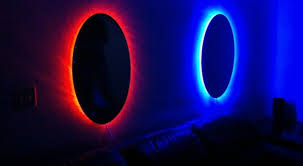
\includegraphics[scale=0.70]{imagenes/portales1.jpeg}
      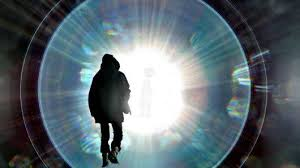
\includegraphics[scale=0.70]{imagenes/portales2.jpeg}
  \end{center}
  \caption{Portales del 2048}
  \label{nCte}
\end{figure}

Los cambios que se realizaron son los siguiente: \newline
\begin{itemize}
	\item La cantidad de pisos es N y todos los pasillos miden L unidades de longitud.
	\item Los portales sirven tanto para ascenso como para descenso de un piso a otro piso(tal piso podría ser el mismo).
	\item Los paracaídas quedaron pasado de moda (obsoletos), por lo tanto ya no sera necesario bajar hasta el piso_0  para volver a intentar subir cuando nos equivoquemos.
	\item Como dijimos cada pasillo tiene largo L, dónde a cierta distancia desde origen podrán estar ubicados los portales.
	\item Cada portal nos transportara a otro piso a una cierta distancia del origen del pasillo (tal vez el mismo piso pero a distinta distancia).
	\item Se asegura que en toda instancia del problema es posible realizar el recorrido deseado, y que no hay más de un portal que comunique las mismas posiciones del mismo par de pisos. Observar que puede haber mas de un portal que comuniquen el mismo par de pisos, y portales que comuniquen posiciones diferentes dentro del pasillos de un mismo piso.
	\item El alumno parte siempre del piso_0 y quiere llegar al piso_N donde la puerta del salon esta ubicada al final del pasillo. 
\end{itemize}


 
\textbf{Problema concreto a resolver:} \newline

Todos nuestros estudiantes son muy aplicados, tanto que necesitan llegar de la manera mas rápido(rapidez en tiempo) al aula donde se dicta la materia de  Algoritmos y estructuras de datos III, con lo idea de llenar de consultas a los docentes y presenciar sus clases magistrales. Estos alumnos están muy confundidos con las nuevas funcionalidades de los portales ya descriptos arriba.
El problema consiste en llegar en el menor tiempo posible al aula(piso_N al final del pasillos), osea queremos optimizar el tiempo(en esta caso minimizar tiempo).
Hay que tener cuenta ciertas cosas, para eso voy a dar un poco de notación, condiciones iniciales y finales.
\begin{itemize}
	\item A, $D_A$: B , $D_B$ que indica que el portal $A$ esta Adistancia $D_A$ del pasillo de inicio del piso A, y  te transporta hasta el piso B dónde la salida del portal esta a distancia $D_B$.
	\item Recordar que el alumno siempre comienza desde el piso_0 a distancia cero del pasillo.
	\item Estos alumno tienen como objetivo llegar hasta el piso_N a distancia L, que es justo donde queda la puerta de entrada al salón.
	\item Recorrer 1 metro del pasillo requiere de 1 segundo y utilizar el portal nos demanda 2 segundos(en cualquiera de las dos direcciones). 	 
\end{itemize}
 Damos ejemplo para aclarar como tenemos la entrada y que queremos de salida (input y output).
 Notar que cada portal va estar identificado como una 4-upla  de la siguiente manera $(A,D_A,B,D_B)$. Los valores A, D_A, B y D_B son los mismos que enunciamos mas arriba. 
 \newline
Ejemplo 1:
\begin{figure}[H]
 \begin{center}
     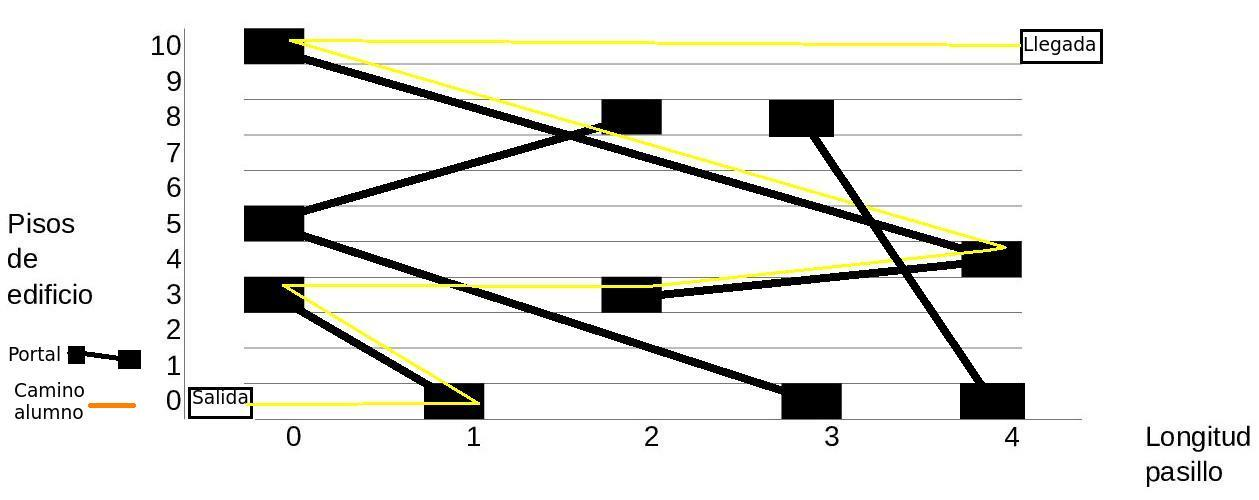
\includegraphics[scale=0.30]{imagenes/ejercicio2ej1.jpg}
 \end{center}
 \caption{ 6 portales, 10 pisos, 4 unidades de longitud de pasillo}
 \label{nCte}
\end{figure}

\begin{itemize}
	\item Entrada : \{ (0,1,3,0),(0,3,5,0)(0,4,8,3)(3,2,4,4)(5,0,8,2)(4,4,10,0)\}
	\item Salida : 13 , que es la cantidad mínima de tiempo que el alumno tarda en llegar al aula(Ver las lineas amarillas del gráfico) 
\end{itemize}

Ejemplo 2: \newline
\begin{figure}[H]
 \begin{center}
     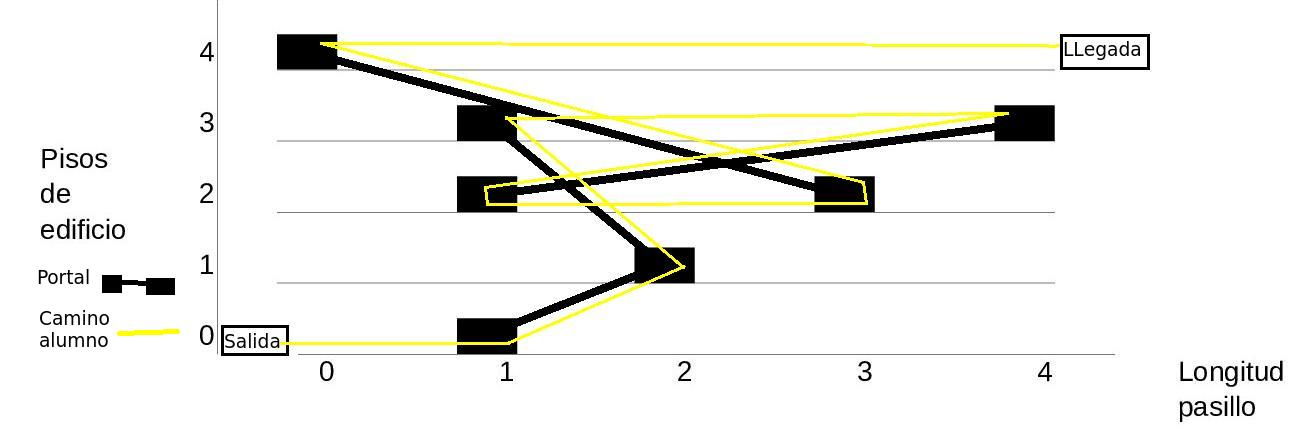
\includegraphics[scale=0.30]{imagenes/ejercicio2ej2.jpg}
 \end{center}
 \caption{ 4 portales, 4 pisos, 4 unidades de longitud de pasillo}
 \label{nCte}
\end{figure}

\begin{itemize}
	\item Entrada : \{ (0,1,2,2),(1,2,3,1),(2,1,3,4),(2,3,4,0)\}
	\item Salida : 18 , que es la cantidad mínima de tiempo que el alumno tarda en llegar al aula(Ver las lineas amarillas del gráfico) 
\end{itemize}
 
%\textbf{completar!}

\subsection{Desarrollo de la idea y pseudocódigo.}

Utilizamos el siguiente procedimiento para obtener la mínima cantidad de segundos necesaria para hacer el recorrido:
Modelamos cada piso de $ L $ metros con $ L+1 $ nodos, y cada portal como un nodo enlazado a los nodos correspondientes según que pisos/metros una. De esta forma podemos considerar que el tiempo que se tarda en ir de un nodo a otro es $1~s$. Para atravesar por un portal hay que pasar por un nodo intermedio, por lo que se gastan $2~s$, en cambio para recorrer un metro, solo $1~s$.

En base a esto implementamos una modificación de $ BFS $, para calcular la distancia entre el nodo correspondiente al metro cero del primer piso, y el correspondiente al último metro del último piso. Para la misma utilizamos una clase especial para los nodos, la cual incluye los atributos $ distancia $ de tipo int, $  marcado$ de tipo bool, $ sucesores $, la cual es una lista de nodos con los sucesores, para la misma consideramos que un nodo es sucesor de otro si están unidos por una arista en el grafo, ya que los portales son bidireccionales, y en los pasillos es posible avanzar y retroceder. Por ultimo los nodos tienen el atributo $ id $ de tipo int, el cual es un número que identifica unívocamente cada nodo. Para los nodos utilizamos los números para identificarlos en orden, es decir, para el primer piso  los números de cero a $ L $, par los del segundo de $ L+1 $ a $ 2L+1 $. y así siguiendo. Para los nodos correspondientes a los portales utilizamos los números siguientes a los ya utilizados para los nodos de los pasillos.

Implementamos en java el algoritmo de $ BFS $ dado en la teórica \cite{teorica}, con la diferencia de que va completando el atributo distancia. Cada vez que se descubre un nuevo nodo se le asigna una distancia de 1 + la distancia de su antecesor, y también se pregunta si su atributo $ id $ es $(N+1)*(L+1)-1)$, en ese caso termina de ejecutar. La solución fue implementada en una clase de java llamada $ Ejercicio2 $.



\subsection{Correctitud}

Para garantizar que nuestro algoritmo es correcto, tiene que valer que el camino que encuentra por primera vez el último nodo, sea el de menor longitud. Esto es verdadero, ya que el algoritmo de $ BFS $, recorre los nodos con distancias en orden, es decir primero los que están a distancia 1, luego los que están a distancia 2, y así siguiendo. Esto se debe a que el algoritmo empieza con un elemento inicial en la cola ''First-in, First-out'', luego encola los sucesores del mismo, los cuales están a distancia uno. Entonces va desencolando de a uno los elementos de la cola y encolando sus sucesores, los cuales están a distancia dos. Como los que primero ingresan son los primeros que salen, primero salen de la cola, los nodos a distancia cero, luego los a distancia uno, dos, y así sucesivamente.


\subsection{Análisis de complejidad}

%\vspace*{0.3cm}

%\textbf{completar!}

Se calcularan las complejidades en base los parámetros de entrada cantidad de portales, denotado por $ P $ , piso mas grande, denotado por $ N $, y cantidad de metros de los pasillos denotado por $ L $.

La complejidad de este algoritmo depende del número de iteraciones antes de encontrar el nodo buscado, para una instancia aleatoria particular, la complejidad dependerá de la configuración de los portales.
El peor caso es cuando se visitan todos los nodos. Analizamos la complejidad en peor caso, en el código del apéndice.  Como en todo algoritmo $bfs$, sobre un grafo, tiene un complejidad en peor caso de $O(n+m)$, donde n es la cantidad de nodos, y m la cantidad de aristas. En este caso tenemos $n=(N+1)*(L+1) +P$, y $m= (N+1)*(L) +2P$, con lo que tenemos una complejidad de $O(N*L+P)$ en peor caso.

El mejor caso es cuando los nodos inicial y final pueden estar conectados por un portal, por lo que la complejidad de la misma será la misma que para elaborar el grafo, la cual es $ O(N*L+P) $ tal como puede verse en el apéndice.


\subsection{Experimentación}

Para generar instancias en peor caso utilizamos la clase $ GenereadorInstanciasEj2 $,el cual al ejecutarse, genera un archivo llamado $ Ej2Instancias.in $ con aquellas. Las mismas consisten en unir los pisos contiguos, por ejemplo el cero con el uno, por medio de portales que comuniquen la baldosa $ L $ de un piso con la cero 
del siguiente. De esta manera para llegar desde el punto de partida al final, se necesitan recorrer todos los metros de todos los pasillos, y pasar por todos los portales, que en este caso tenemos $ P=N $. Si calculamos el resultado esperado en segundos según este recorrido obtenemos: $ Tiempo=(N+1)L+2N $. Se podría demostrar que para esos parámetros de $ N $, $ L $ y $ P $ esa configuración corresponde al peor caso.

Para ese tipo de instancias, se consideraron dos experiencias. En una se deja fijo la cantidad de baldosas $ L $, y se varia la cantidad de pisos, $ N $, con la cual también varia la cantidad de portales $ P $, ya que se mantiene invariante que $ P=N $. En la otra experiencia, se deja fijo $ N $ y $ P $, y se varia $ L $. 

Para tomar tiempos se utilizo la clase $ Ej2Tiempos $, en la cual para cada instancia se corre 600 veces el algoritmo se guardan los resultados en un arreglo. Calculamos el promedio  y el desvío estándar del mismo, y luego lo filtramos quedándonos con los valores que estuvieran entre el promedio menos el desvío estándar y promedio mas el desvío estándar. Finalmente tomamos un promedio de los valores que quedaron, y ese es el resultado que consideramos como tiempo final.

En las figuras~\ref{peorCasoNfijo} y \ref{peorCasoLfijo} podemos ver los resultados obtenidos.

\begin{figure}[H]
\centering
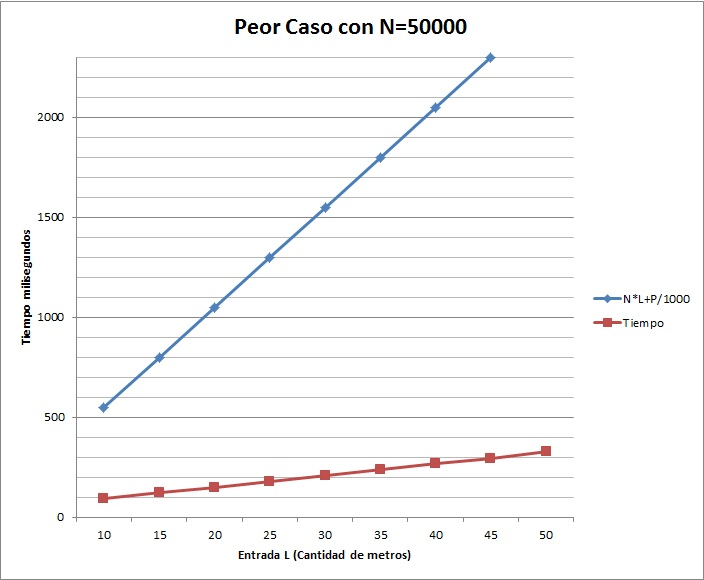
\includegraphics[scale=0.6]{../PeorCasoEj2Nfijo.jpg}
\caption{Gráfico de tiempos obtenidos en función de $L$, para valores de $ N $ y $ P $ fijos en 50000, con una configuración de peor caso para estos tres parámetros.}
\label{peorCasoNfijo}
\end{figure}

En la figura~\ref{peorCasoNfijo} se puede visualizar como el tiempo de computo varia linealmente con $ L $, tal como es de esperarse teóricamente.
\begin{figure}[H]
\centering
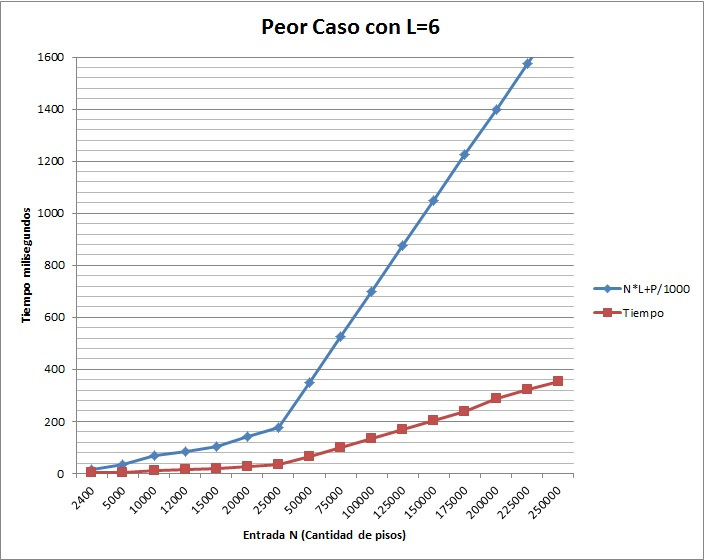
\includegraphics[scale=0.6]{../PeorCasoEj2Lfijo.jpg}
\caption{Gráfico de tiempos obtenidos en función de $N$, para un valor de $ L $  fijo en 6, con una configuración de peor caso para los tres parámetros.}
\label{peorCasoLfijo}
\end{figure}

En la figura~\ref{peorCasoLfijo} se puede visualizar como el tiempo de computo varia según el parámetro $ N $ de la configuración. Podemos distinguir que se comporta en forma similar a la función utilizada para comparar a la misma, la cual se encuentra en la misma figura.

Para el mejor caso se consideraron las instancias ya utilizadas en el peor caso(notar que tienen mismo $ N $, $ L $ y $ P $), pero con la modificación de que el punto inicial con el final estén conectados por un portal, de esta manera el resultado esperado es de dos segundos. Para generar estas instancias utilizamos la clase $ GeneradorInstanciasMejorCaso $, el cual al ejecutarse produce el archivo $ Ej2InstanciasMejorCaso.in $. Nuevamente tomamos tiempos con la clase $ Ej2Tiempos $. En las figuras~\ref{mejorCasoNfijo} y \ref{mejorCasoLfijo} podemos ver los resultados obtenidos.

\begin{figure}[H]
\centering
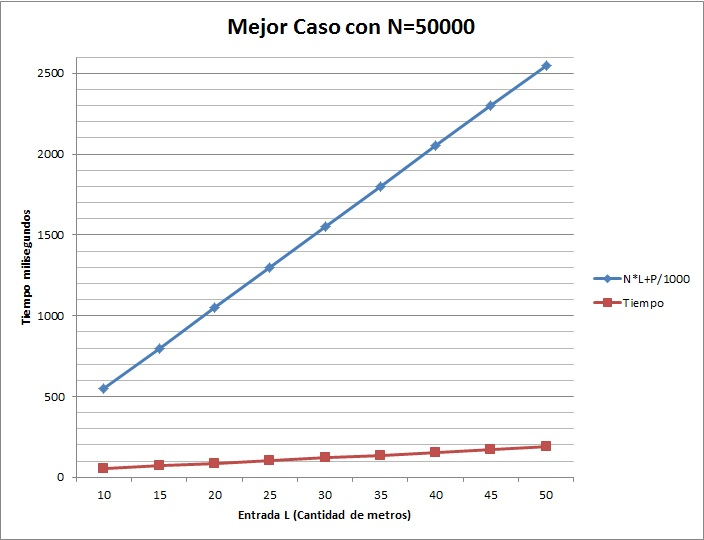
\includegraphics[scale=0.6]{../MejorCasoEj2Nfijo.jpg}
\caption{Gráfico de tiempos obtenidos en función de $L$, para valores de $ N $ y $ P $ fijos en 50000, con una configuración de mejor caso para estos tres parámetros.}
\label{mejorCasoNfijo}
\end{figure}

\begin{figure}[H]
\centering
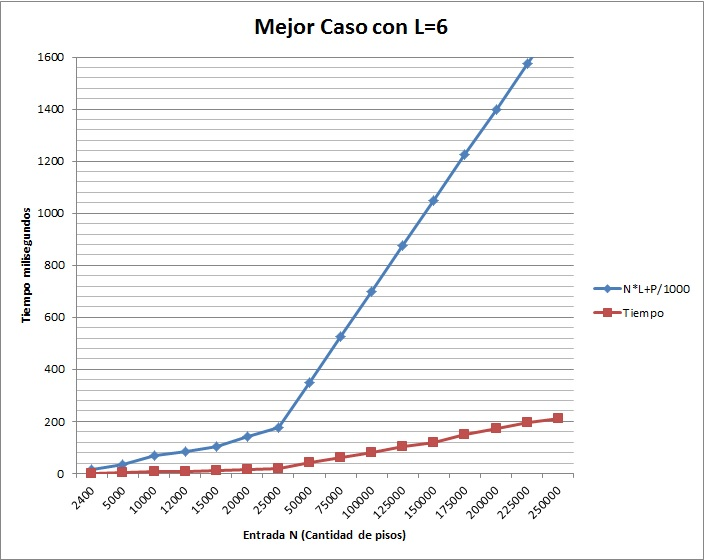
\includegraphics[scale=0.6]{../MejorCasoEj2Lfijo.jpg}
\caption{Gráfico de tiempos obtenidos en función de $N$, para un valor de $ L $  fijo en 6, con una configuración de mejor caso para los tres parámetros.}
\label{mejorCasoLfijo}
\end{figure}

En las figuras~\ref{mejorCasoNfijo} , y \ref{mejorCasoLfijo} podemos ver como el tiempo de computo varia en función de los parámetros para una configuración de mejor caso, en forma análoga a como varia para una de peor caso.

Para el caso aleatorio se generaron instancias con la clase $ GeneradorInstanciasAleatorioMismo $, el cual al ejecutarse las guarda las mismas en $ Ej2InstanciasAleatorioMismo.in $. Se utilizaron los mismos valores de $ N $, $ L $ y $ P $, pero con la particularidad que los pisos y baldosas comunicados se seleccionan aleatoriamente. Se utilizo la clase Random de java con semilla fijada en 55 para generar números aleatorios.

Para constatar que la las instancias aleatorias lleguen al piso deseado, se hizo una modificación de la clase $ Ejercicio2 $, para que en caso de que se encuentre al mismo, imprima por pantalla ''Encontrado'' junto con los valores de $ L $ y $ N $, y así poder identificar si la instancia generada aleatoriamente es valida. En caso de no ser valida, se gasta un $ nextInt $ almacenándolo en una variable extra llamada $ nop $ creada con tal propósito. De esta manera los valores que se obtienen aleatoriamente y se imprimen en el archivo son distintos, obteniendo una nueva instancia(distinta a la que se obtendría sin gastar un $ nextInt $ extra) que posiblemente sea valida. Se repite el procedimiento hasta conseguir que la instancia sea valida, y esto se repite para cada instancia, consiguiendo que todas las instancias generadas sean validas.

En las figuras~\ref{aleatorioCasoNfijo} y \ref{aleatorioCasoLfijo} podemos ver los resultados obtenidos.

\begin{figure}[H]
\centering
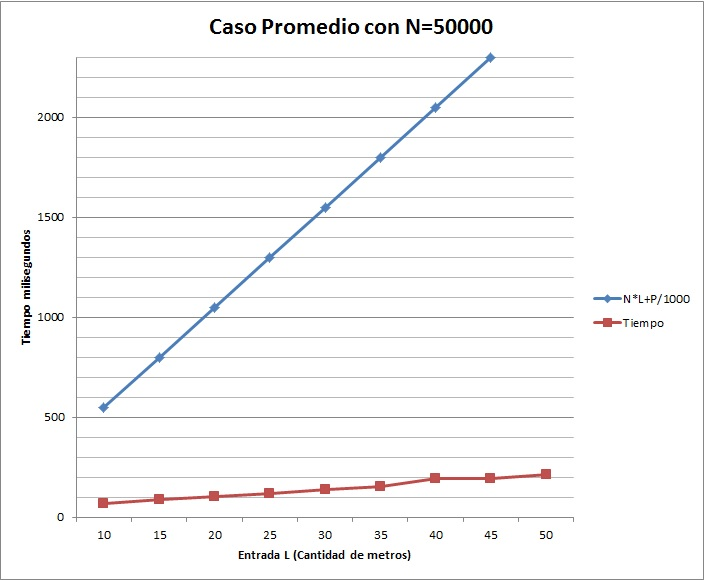
\includegraphics[scale=0.6]{../CasoPromedioEj2Nfijo.jpg}
\caption{Gráfico de tiempos obtenidos en función de $L$, para valores de $ N $ y $ P $ fijos en 50000, con una configuración aleatoria para estos tres parámetros.}
\label{aleatorioCasoNfijo}
\end{figure}

\begin{figure}[H]
\centering
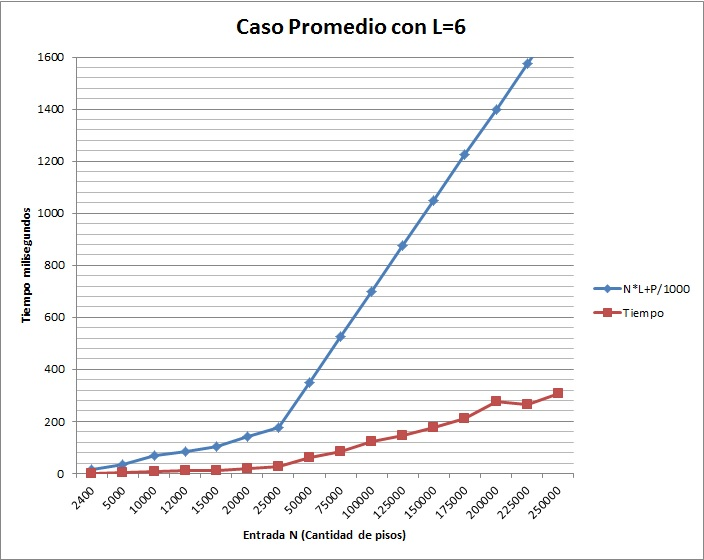
\includegraphics[scale=0.6]{../CasoPromedioEj2Lfijo.jpg}
\caption{Gráfico de tiempos obtenidos en función de $N$, para un valor de $ L $  fijo en 6, con una configuración de mejor caso para los tres parámetros.}
\label{aleatorioCasoLfijo}
\end{figure}

En las figuras~\ref{aleatorioCasoNfijo} y \ref{aleatorioCasoLfijo} podemos distinguir que para configuraciónes aleatorias de $ N $, $ L $ y $ P $, las funciones varían en forma ''similar''' al peor y mejor caso, aunque difieren en no tener un comportamiento tan uniforme.

En cuanto a la comparación entre el tiempo de computo de peor, mejor y caso aleatorio, a pesar de tener el mismo orden de complejidad, en las experiencias se pudo distinguir claramente como las instancias de peor caso tienen un tiempo mayor, seguidas por la de caso aleatorio y por último las de mejor caso. En las figuras \ref{ComparacionCasoNfijo} y \ref{ComparacionCasoLfijo} podemos comparar los tiempos de computo para peor y mejor caso.


\begin{figure}[H]
\centering
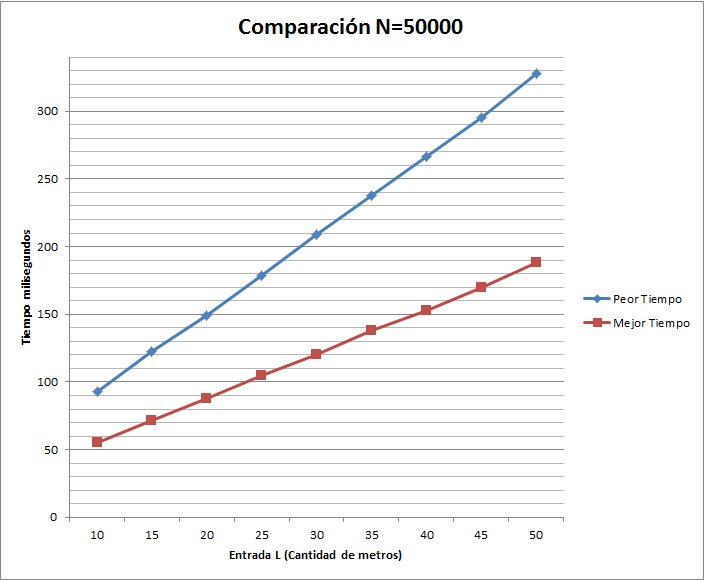
\includegraphics[scale=0.6]{../ComparacionEj2Nfijo.jpg}
\caption{Gráfico de tiempos obtenidos en función de $L$, para valores de $ N $ y $ P $ fijos en 50000, con una configuración de peor y mejor caso para estos tres parámetros.}
\label{ComparacionCasoNfijo}
\end{figure}

\begin{figure}[H]
\centering
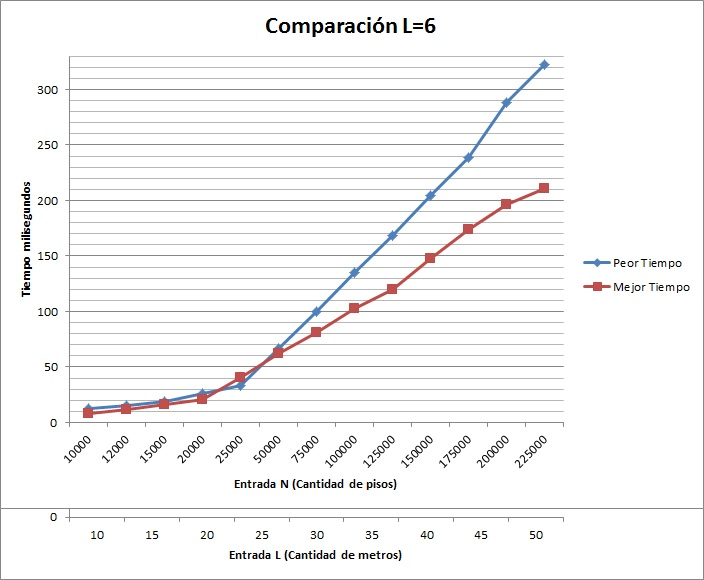
\includegraphics[scale=0.6]{../ComparacionEj2Lfijo.jpg}
\caption{Gráfico de tiempos obtenidos en función de $N$, para un valor de $ L $  fijo en 6, con una configuración de peor y mejor caso. }
\label{ComparacionCasoLfijo}
\end{figure}




\subsection{Validación}

Para validar el algoritmo, utilizamos los casos de test de la cátedra, y también se verificó que el resultado para las instancias de mejor y peor caso utilizadas en la experimentación sea el esperado.

En el archivo $ ResultadosEsperadosPeorCasoEj2.ods $ podemos encontrar los resultados esperados para el peor caso, y para el mejor caso sabemos que tienen que ser todos dos.

